\section{Periodograms from various sources of data}
\protect\label{section:variousrot}

Using data from the various papers referred to above, attempts were made to
recover periodic data from the various sources referred to and also from data
associated with the goal of this project, the {\rem} telescope.

\subsection{Study of data from \ktwo}
\protect\label{section:k2data}

Data from {\ktwo} was only available for a single 80-day period starting on 15
October 2005. This showed an interval at the start strongly affected by frequent
flaring events, however there was a quiescent period during which a regular
cyclic pattern could be observed, for example as seem in
Fig. \ref{fig:k2all} with the latter part in Fig. \ref{fig:k2lcurve}.
This last part shows a clear periodic cycle
which can be used to generate a very clear periodogram as shown in Fig.
\ref{fig:k2pgram}, with a very prominent peak at 2.87 days. A light curve folded
on this period is shown in Fig. \ref{fig:k2pfold}. The display starts at 2 days,
as the window function of the time series, as shown in Fig. \ref{fig:k2winfunc},
shows significant peaks in the periods below this.

\begin{figure}[!htbp]
\begin{center}
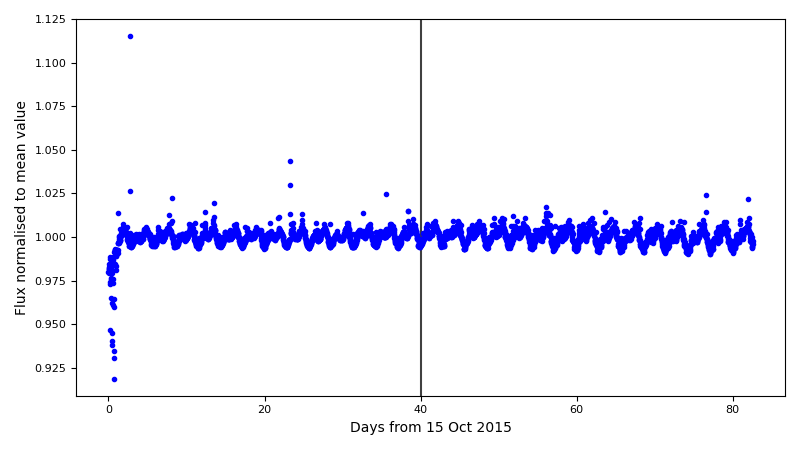
\includegraphics[scale=0.40]{k2/images/k2all.png} \\
\vspace{-.5cm}
\end{center}   
\caption{Scatter plot of observed flux for {\ross} taken from the archive of
{\ktwo} data on MAST for 10 October 2015 onward. The error bar is too small to
display. The first part appears to be affected by some diminution in activity or
error and in subsequent analysis, the portion to the right of the vertical line
set at 40 days is taken.}\protect\label{fig:k2all}
\end{figure}

\begin{figure}[!htbp]
\begin{center}
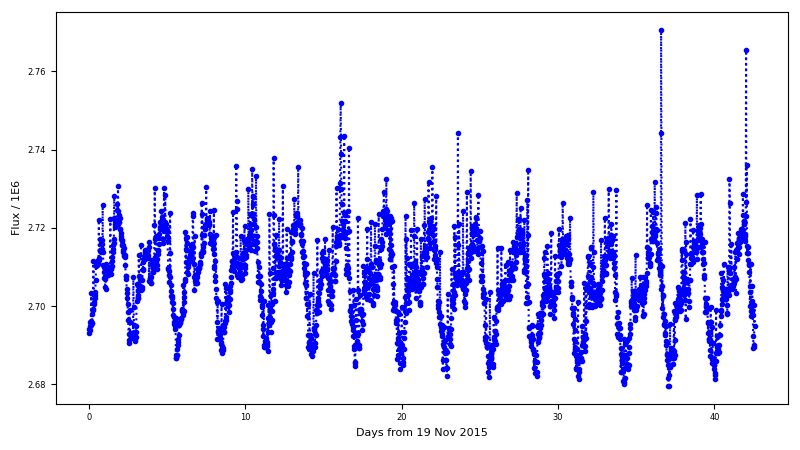
\includegraphics[scale=0.40]{k2/images/k2lcurve.png} \\
\vspace{-.5cm}
\end{center}   
\caption{Scatter plot of observed flux for {\ross} taken from the archive of
{\ktwo} data on MAST for 10 October 2015 onward, omitting the first 40 days,
which appear, especially at the beginning, to be affected by a significant
reduction in activity, and also outlying data of greater than 2 standard deviations.
Again, the error bar is too small to display.}\protect\label{fig:k2lcurve}
\end{figure}

\begin{figure}[!htbp]
\begin{center}
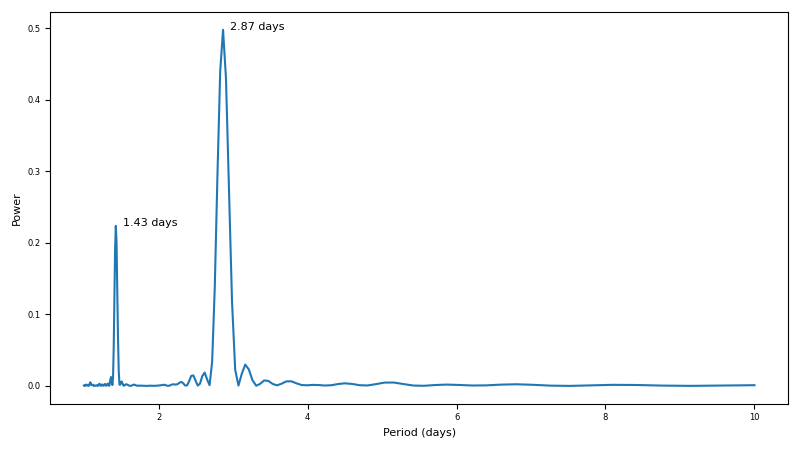
\includegraphics[scale=0.40]{k2/images/k2_pg.png} \\
\vspace{-.5cm}
\end{center}   
\caption{Periodogram taken from the data displayed in Fig.
\ref{fig:k2lcurve} but not omitting outlying data
greater than 2 standard deviations, which made
little difference to the result. There were additional peaks of less than a day
to be observed, however these have been omitted as there were aliases of the
2.87 day period, observed from the emulations described below, which conflicted
with these.} \protect\label{fig:k2pgram}
\end{figure}

\begin{figure}[!htbp]
\begin{center}
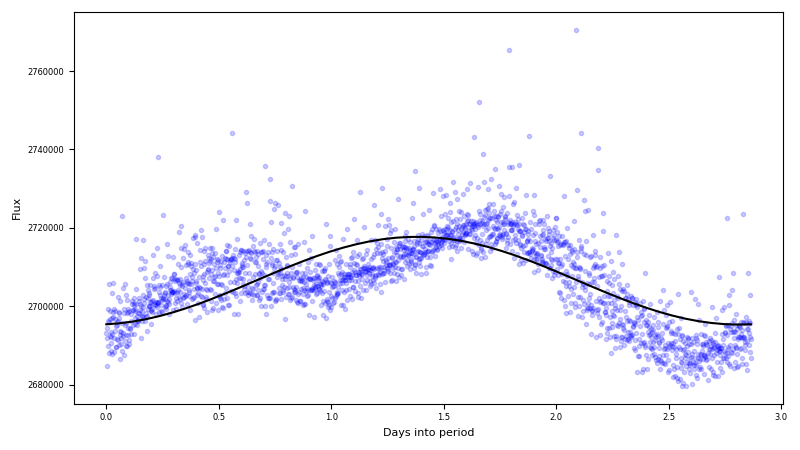
\includegraphics[scale=0.40]{k2/images/k2_pfold.png} \\
\vspace{-.5cm}
\end{center}   
\caption{Light curve taken from the data displayed in Fig.
\ref{fig:k2lcurve} folded on the main peak of 2.87 days displayed in Fig.
\ref{fig:k2pgram}. Points exceeding 2 standard deviations from the mean are
omitted for clarity of display.} \protect\label{fig:k2pfold}
\end{figure}

\begin{figure}[!htbp]
\begin{center}
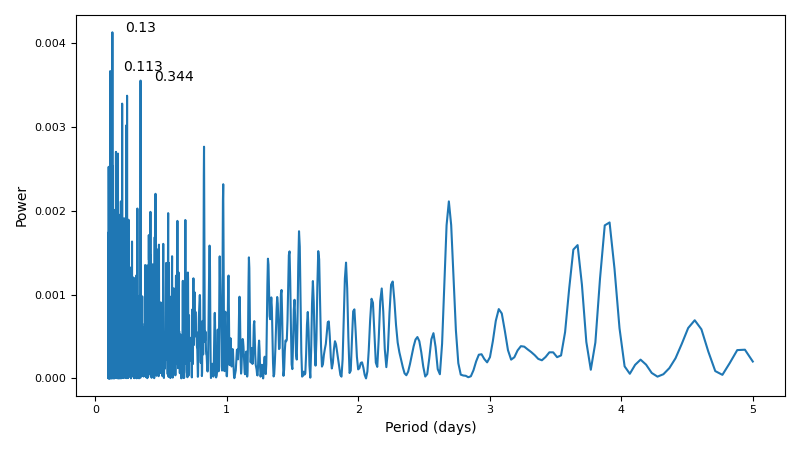
\includegraphics[scale=0.40]{k2/images/k2winfunc.png} \\
\vspace{-.5cm}
\end{center}   
\caption{Window function of the time series for the {\ktwo} data showing numerous
peaks in the period space below 2 days.} \protect\label{fig:k2winfunc}
\end{figure}

On the hypothesis that there were patterns of bright or dark spots on the face
of {\ross} which were relatively static over a period of a few days, like the
Sun, a very simple model, using the same time parameters as with Fig.
\ref{fig:k2lcurve} and Fig. \ref{fig:k2pgram}, was run yielding the result in
Fig. \ref{fig:k2emulated}. Results, as will be apparent, were virtually
identical to those from the {\ktwo} data for \ross, even though the simulated
noise on the values for the flux was ramped up to worse than 50 to 1, far worse for
that for the {\ktwo} data, the mean SNR of which was better than 40,000 to 1.
Whatever pattern on light or dark data, other than artificially cyclical data,
yielded the same periodogram.

Both the ``real'' periodogram and the emulated one showed strong peaks of less
than 1 day which have to be aliases of the 2.87 period and prevent any
meaningful analysis of periods less than 1 day which might be suggested by the
format of the cycles observed in Fig. \ref{fig:k2lcurve}.

\begin{figure}[!htbp]
\begin{center}
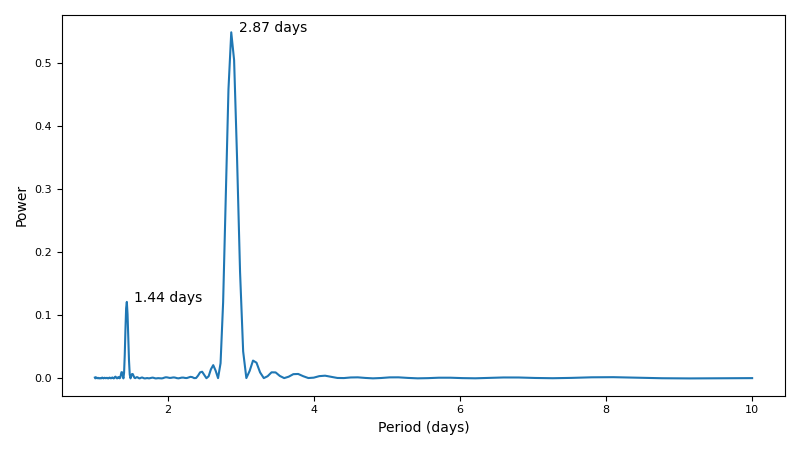
\includegraphics[scale=0.40]{k2/images/k2emulated.png} \\
\vspace{-.5cm}
\end{center}   
\caption{Periodogram generated by using the same time periods as shown in Fig. \ref{fig:k2lcurve} and
for which a periodogram is shown in Fig.
\ref{fig:k2pgram} but with simulated spot data over the surface and assuming a
rotation period of 2.87 days. Gaussian noise of 2\% of the signal level was
added to the data, although this is far worse
than with the {\ktwo} data used in the preceding
figures. Even without the noise, there were
aliases observed of the 2.87 day period of less
than 1 day which obscured any periodogram
obtainable, as shown in Fig. \ref{fig:k2winfunc}, which is why periods of less
than 1 day were omitted from this figure and also from
Fig. \ref{fig:k2pgram}.}\protect\label{fig:k2emulated}
\end{figure}

It would appear that this is the rotation period being tracked by surface
features. One might expect to see the surface features evolve over time and
worth checking if such changes have any significant effect on the periodogram
results. In Fig. \ref{fig:win20day} the periodogram was recalculated from a
20 day window with successive starting periods over the same data in Fig.
\ref{fig:k2pgram}, showing the variations on the two mean peaks which result.
In Fig. \ref{fig:k2winsizes} is shown the variations in the periodogram result
taking various sizes of window.

\begin{figure}[!htbp]
\begin{center}
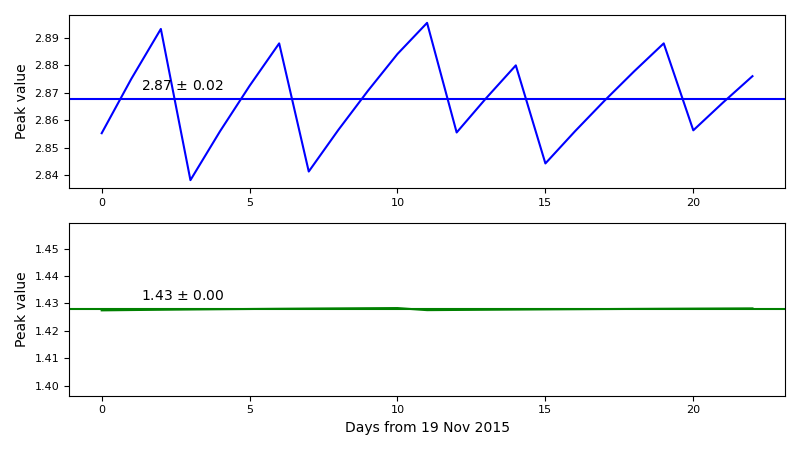
\includegraphics[scale=0.40]{k2/images/period_track.png} \\
\vspace{-.5cm}
\end{center}   
\caption{This shows the variations in the result from the first two peaks
(represented as blue and green) in the periodogram shown over the whole of the
data for the last 40 days (19 November 2015 onward) by taking a 20-day
``window'' of the data starting at successive days.
The scale is kept at the same value for both plots
for comparison.}\protect\label{fig:win20day}
\end{figure}

\begin{figure}[!htbp]
\begin{center}
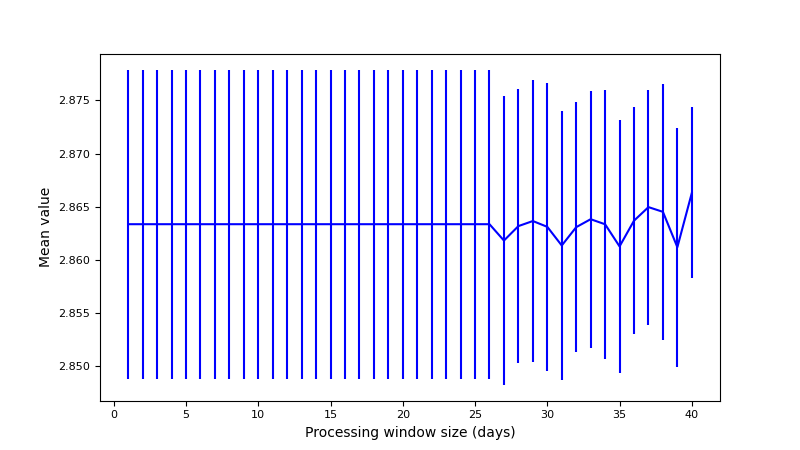
\includegraphics[scale=0.40]{k2/images/k2winsizes.png} \\
\vspace{-.5cm}
\end{center}
\caption{This shows the mean value of the
periodogram main peak (solid line) and the
standard deviations (dotted line, scale on RH
axis), for successive window sizes with the
windows run over the whole data from 19 November
2015.}\protect\label{fig:k2winsizes}
\end{figure}

It would appear that consistent results showing a rotation period of 2.87 $\pm$
0.01 days are obtainable from {\ktwo} and also a ``window'' of up to 20 days is
suitable without errors being introduced due to changes to the surface features.
For any set of data, there will have to be a compromise between the frequency
of observations in a set and minimising the number of days over which the sample is taken.
{\ktwo} has approximately 50 observations recorded each day which is more than enough
to obtain a result over just one day, given the excellent SNR.
